%versi 2 (8-10-2016)
\chapter{Landasan Teori}
\label{chap:teori}
Pada bab ini akan dijelaskan mengenai Google VR, Google StreetView API, Google Directions API, dan \textit{motion sensor}.

%GOOGLE VR
\section{Google VR}
\label{sec:google-vr} 
Google VR adalah teknologi yang diciptakan perusahaan Google untuk membuat pemandangan dunia maya yang terlihat nyata dengan menempatkan \textit{smartphone} pada alat yang bernama \textit{viewer} ~\cite{quickstart-google-vr}. \textit{Viewer} adalah alat untuk melihat dunia VR pada aplikasi VR di \textit{smartphone}. Dua \textit{viewer} yang diciptakan Google adalah \textit{Google Daydream} dan \textit{Cardboard}. Perbedaan dari \textit
{Google Daydream} dan \textit{Google Cardboard} adalah pada bahan dan alat penerima masukan (\textit{input}). \textit{Google Daydream} memiliki alat penerima masukan pengguna seperti \textit{remote control} dengan beberapa tombol serta berbahan utama plastik, sedangkan \textit{Google Cardboard} memiliki penerima masukan berupa satu tombol (biasanya berupa magnet) yang akan memicu terjadinya suatu \textit{event} dan berbahan dasar kardus. Google menyediakan sebuah alat bantu bagi pengembang perangkat lunak untuk memudahkan pengembangan aplikasi VR yang disebut Google VR SDK.

\subsection{Google VR SDK}
Google VR SDK adalah alat bantu berlisensi Apache 2.0 yang disediakan Google pada repository Github yang berisi kode program dari aplikasi {\it virtual reality} (VR)  yang tersedia untuk Android (Java), Android NDK, Unity, dan iOS ~\cite{all-google-vr}. Secara umum, SDK ini dibuat agar pengembang perangkat lunak dapat mempelajari serta memanfaatkan teknologi VR yang disediakan Google ~\cite{quickstart-google-vr}. Ada beberapa aplikasi yang tersedia pada SDK tersebut seperti aplikasi demo bernama HelloVR dan pemutar video dalam VR, tetapi penulis akan memanfaatkan bagian aplikasi demo HelloVR untuk Android Java pada Google VR SDK. Untuk menggunakan SDK ini, dibutuhkan perangkat lunk Android Studio 2.3.3 dan lebih tinggi, dengan Android SDK versi 7.1.1 (API Level 25) atau lebih tinggi. Gambar \ref{fig:gvr-dir} menunjukkan struktur \textit{folder} dari Google VR SDK untuk Android.

\begin{figure}[h]
	\centering
		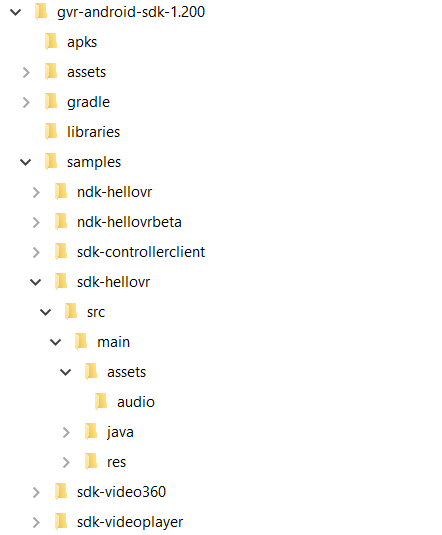
\includegraphics[scale=1.0]{Gambar/gvr_dir.png}
	\caption{Struktur Direktori Google VR SDK}
	\label{fig:gvr-dir}
\end{figure}

Google menyediakan \textit{library} untuk bahasa pemrograman Java pada \textit{package} \texttt{com.google.vr.sdk.base} agar dapat digunakan pengembang perangkat lunak untuk membuat aplikasi VR ~\cite{google-vr-sdk}. Berikut adalah beberapa \textit{class} dan \textit{interface} dari \textit{package} \texttt{com.google.vr.sdk.base}:

	\begin{enumerate}
		\item \texttt{GvrView.StereoRenderer}
		
		\textit{Interface} untuk \textit{renderer} yang menyerahkan seluruh penyajian pemandangan stereo pada pemandangan (\textit{view}). \textit{Method-emethod} abstrak yang dimiliki \textit{interface} imi adalah:
			\begin{itemize}

				\item \texttt{public abstract void onDrawEye (Eye eye)}
				
\textit{Method} yang menggambar pemandangan untuk satu mata. \textit{Method} ini tidak memiliki nilai yang dikembalikan ataupun\textit{exception}. 

				\item \texttt{public abstract void onFinishFrame (Viewport viewport)}
\textit{Method} yang dipanggil sebelum \textit{frame} selesai dibuat. Parameter yang dimiliki \texttt{method} ini adalah:
				\begin{itemize}

					\item \texttt{Viewport viewport}: \textit{Object viewport} yang dari GL \textit{surface}.
				\end{itemize}
				
\textit{Method} ini tidak memiliki nilai yang dikembalikan ataupun\textit{exception}.
				
				\item \texttt{public abstract void onNewFrame (HeadTransform headTransform)}				
\textit{Method} untuk menggambar perubahan \textit{frame} dari pemandangan. Parameter yang dimiliki \texttt{method} ini adalah:

				\begin{itemize}
					\item \texttt{HeadTransform headTransform}: 						\textit{Object} dari kelas \textit{headtransform}, yang mendefinisikan perubahan posisi kepala pengguna.  
				\end{itemize}		
				\textit{Method} ini tidak memiliki nilai yang dikembalikan, juga tidak memiliki \textit{exception}. 						
				
				\item \texttt{public abstract void onRendererShutdown()}
\textit{Method} yang dipanggil ketika \textit{thread renderer} dari pemandangan berhenti atau dimatikan, ketika method \texttt{onSurfaceCreated} dipanggil. \textit{Method} ini tidak memiliki parameter, nilai yang dikembalikan, maupun \textit{exception}.
				
				\item \texttt{public abstract void onSurfaceChanged (int width, int height)}
				\textit{Method}	yang terpanggil ketika ada perubahan dimensi pada permukaan dunia VR. Parameter yang dimiliki \textit{method} ini adalah:
				
				\begin{itemize}
					\item \texttt{int width}: Nilai dari lebar pemandangan satu \textit{eye} dalam satuan \textit{pixel}.
					
					\item \texttt{int height}: Nilai dari tinggi pemandangan satu \textit{eye} dalam satuan \textit{pixel}.
				\end{itemize}
				
				\item \texttt{public abstract void onSurfaceCreated (EGLConfig config)}
\textit{Method} untuk membuat dunia VR. Parameter yang dimiliki \textit{method} ini adalah:
				\begin{itemize}
					\item \texttt{EGLConfig config}: Konfigurasi EGL yang digunakan untuk membuat permukaan dunia VR.
				\end{itemize}
			\end{itemize}					
		
		\item \texttt{AndroidCompat}
		
		\textit{Utility class} yang disediakan Android untuk menggunakan fitur-fitur VR.  
			\begin{itemize}
				\item \texttt{public static void setSustainedPerformanceMode (Activity activity, boolean enabled)}
				
\textit{Method} yang mengatur \texttt{android.view.Window} untuk menopang performanya.
				\item \texttt{public static boolean setVrModeEnabled (Activity activity, boolean enabled)}
				
				\textit{Method} ini menyetel pengaturan \textit{VR} yang seseuai untuk suatu \textit{Activity}. Parameter yang dimiliki \textit{method} ini adalah:
				\begin{itemize}
					\item \texttt{Activity activity}
					
					\textit{Activity} yang akan disetel dengan mode VR.
					\item \texttt{boolean enabled}
					
					Nilai \textit{boolean} sesuai dengan apakah mode VR akan diaktifkan atau tidak.
				\end{itemize}
				\item \texttt{public static boolean trySetVrModeEnabled (Activity activity, boolean enabled)}
				
				Sets the appropriate "VR mode" setting for an Activity. Parameter yang dimiliki 
			\end{itemize}					
				
		
		\item \texttt{Eye}
		
		\textit{Class} yang mendefinisikan rincian \textit{rendering} stereo dari satu \textit{eye}. 
			\begin{itemize}
				\item \texttt{public float[] getEyeView ()}
				
				\textit{Method} untuk menghasilkan matriks dari kamera ke \textit{eye}.
				\item \texttt{public FieldOfView getFov ()}
				
				\textit{Method} yang mengembalikan pemandangan untuk satu \textit{eye}.
				\item \texttt{public float[] getPerspective (float zNear, float zFar)}
				
				\textit{Method} untuk mengembalikan matriks proyeksi dari sudut pandang untuk \textit{eye} tertentu.
			\end{itemize}
		
		\item \texttt{GvrActivity}
		\textit{Activity} dasar yang mudah diintegrasikan dengan perangkat Google VR. 
			\begin{itemize}
				\item \texttt{public void onBackPressed ()}
				
				\textit{Method} yang dipanggil ketika tombol kembali ditekan.
				\item \texttt{public void onCardboardTrigger ()}
				
				\textit{Method} yang dipanggil ketika pemicu \textit{Cardboard} ditekan.
				\item \texttt{public void setGvrView (GvrView gvrView)}
				
				\textit{Method} untuk menentukan \texttt{GvrView} pada \textit{activity}. Parameter yang diterima oleh \textit{method} ini adalah:
				
				\begin{itemize}
					\item \texttt{GvrView gvrView}
					
					Objek \texttt{GvrView} yang akan digunakan \textit{activity}.
				\end{itemize}				
			\end{itemize}	 
		
		\item \texttt{GvrView}
		
		\textit{Class} dari \textit{view} yang mendukung VR dari Google. \textit{Method}-\textit{method} yang dimiliki \textit{class} ini adalah:
		
		\begin{itemize}
			\item \texttt{public void setEGLConfigChooser (int redSize, int greenSize, int blueSize, int alphaSize, int depthSize, int stencilSize)}
			
			
		\end{itemize}
		
		\textit{View} yang mendukung \textit{rendering} VR.		
		\item \texttt{HeadTransform}
		
		\textit{Class} yang mendefinisikan perubahan posisi kepala pengguna terhadap dunia VR.
		
		\begin{itemize}
			\item \texttt{public void getEulerAngles (float[] eulerAngles, int offset)}
			
			\item \texttt{public void getForwardVector (float[] forward, int offset)}

			\item \texttt{public void getHeadView (float[] headView, int offset)}
			
			\item \texttt{public void getQuaternion (float[] quaternion, int offset)}
			\item \texttt{public void getRightVector (float[] right, int offset)}
			
			\item \texttt{public void getTranslation (float[] translation, int offset)}
			
			\item \texttt{public void getUpVector (float[] up, int offset)}
		\end{itemize}			
		
		\item \texttt{Viewport}
		\textit{Class} yang mendefinisikan \textit{viewport} berbentuk persegi panjang. 
		
		Atribut-atribut yang dimiliki kelas ini adalah sebagai berikut:
		
		\begin{itemize}
			\item \texttt{public int height}
			
			\item \texttt{public int width}
			
			\item \texttt{public int x}
			
			\item \texttt{public int y}
		\end{itemize}
			
		\textit{Method-method} yang dimiliki kelas ini adalah sebagai berikut:
		
		\begin{itemize}
			\item \texttt{public void getAsArray (int[] array, int offset)}
			
			\item \texttt{public void setGLScissor ()}
			
			\item \texttt{public void setGLViewport ()}
			
			\item \texttt{public void setViewport (int x, int y, int width, int height)}
		\end{itemize}
	\end{enumerate}

\subsection{Aplikasi HelloVR}
\label{subs:hello-vr}
HelloVR, aplikasi yang diperoleh dari Google VR SDK pada direktori \texttt{./samples/sdk-hellovr} adalah sebuah aplikasi demo permainan \textit{treasure hunt}, yaitu sejenis permainan mencari bentuk yang mengapung di dunia VR dengan melihat tepat pada bentuk tersebut dan menyalakan pemicu pada Google Cardboard. Setelah kondisi untuk menangkap bentuk yang ada, bentuk tersebut akan menghilang, lalu bentuk yang lain akan muncul di tempat lain. Gambar \ref{fig:treasure-hunt} menunjukkan tampilan \textit{UI} permainan \textit{treasure hunt} HelloVR. 

\begin{figure}[h]
	\centering
		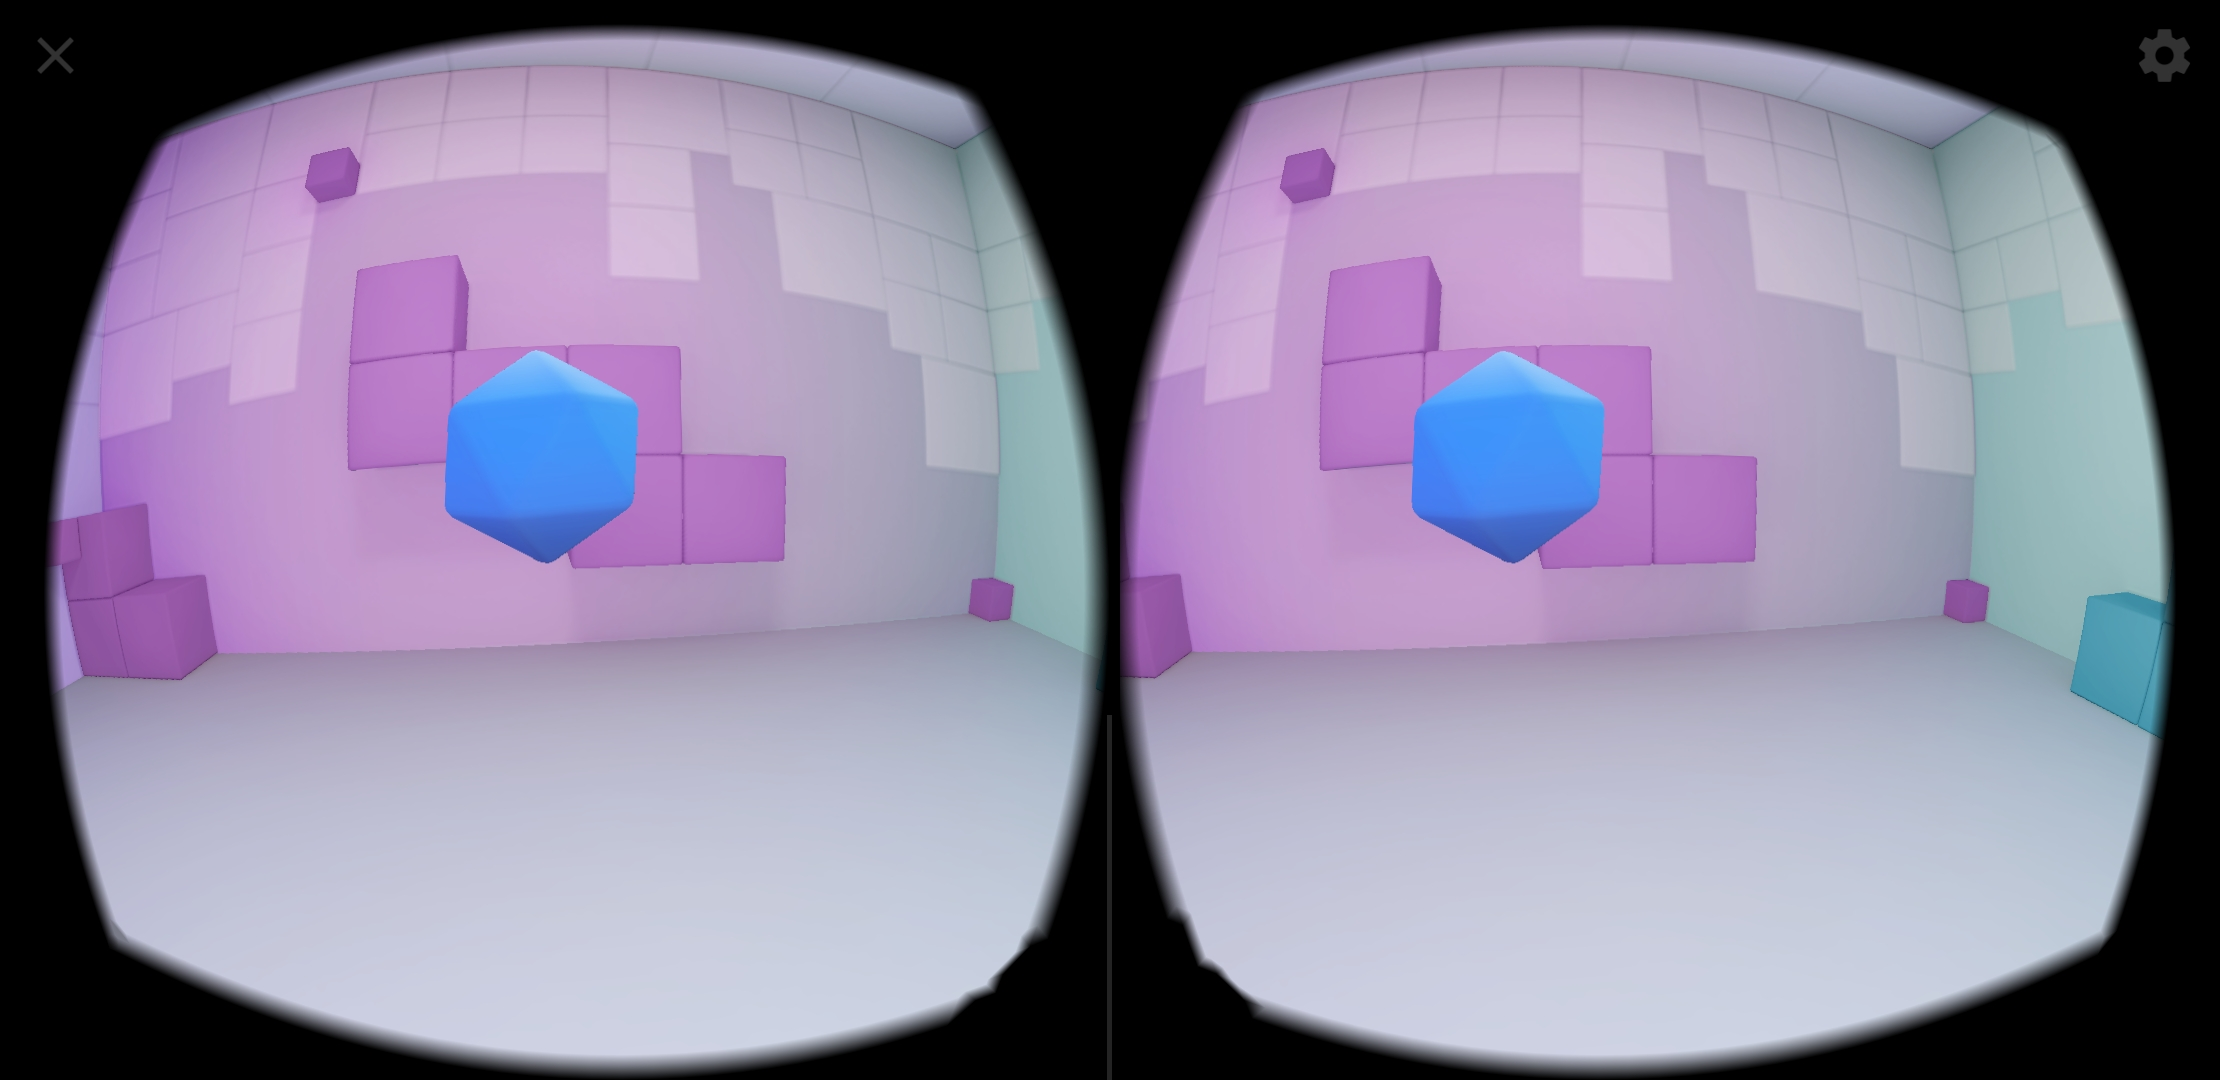
\includegraphics[width=6in]{Gambar/treasure_hunt.jpg}
	\caption{Tampilan \textit{UI} permainan \textit{treasure hunt} pada aplikasi HelloVR}
	\label{fig:treasure-hunt}
\end{figure}

\subsubsection{Komponen Aplikasi HelloVR}
Aplikasi HelloVR terdiri dari beberapa \textit{folder} dan komponen-komponen. Gambar \ref{fig:hello-vr-dir} menunjukkan struktur direktori aplikasi HelloVR. 
Dunia VR pada aplikasi ini dibuat dari {\it file Wavefront Object} (OBJ) dengan tekstur {\it file Portable Network Graphics} (PNG) (Gambar \ref{fig:vr-room}) yang telah dengan sangat tepat dipetakan pada \textit{file} OBJ yang ada sehingga dunia VR terlihat sangat nyata. Bentuk-bentuk yang akan dicari pengguna dibuat dari tiga file OBJ yang merepresentasikan tiga macam bentuk yang akan muncul. Masing-masing file OBJ memiliki dua tekstur yang telah dipetakan pada masing-masing file OBJ dalam file PNG. Satu tekstur (Gambar \ref{fig:blue-shape}) digunakan ketika bentuk sedang tidak ada di tengah-tengah titik pengelihatan pengguna, sedangkan satu tekstur yang lain (Gambar \ref{fig:pink-shape}) digunakan ketika pengguna sedang melihat bentuk tepat di titik tengah pengelihatan pengguna.

\begin{figure}[h]
	\centering
		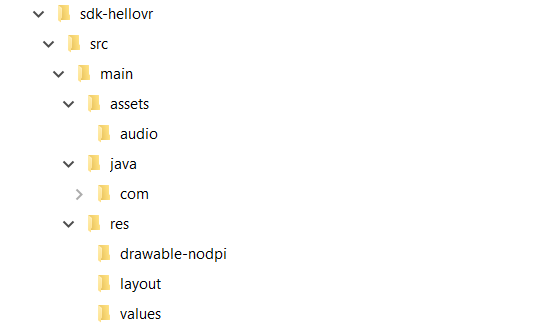
\includegraphics[scale=1.0]{Gambar/hello_vr_dir.png}
	\caption{Struktur Direktori Aplikasi HelloVR}
	\label{fig:hello-vr-dir}
\end{figure}

\begin{figure}[]
	\begin{subfigure}{.33\textwidth}
  		\centering
  		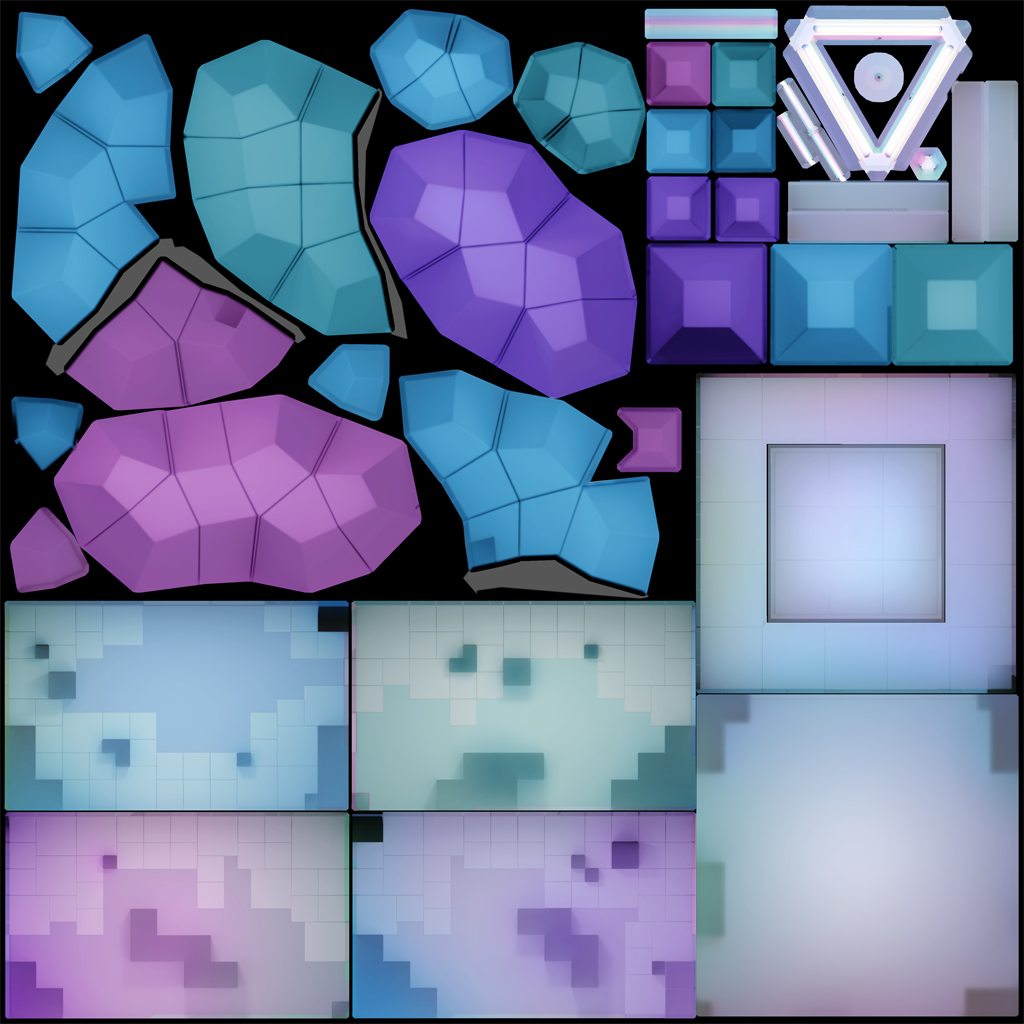
\includegraphics[width=.8\linewidth]{Gambar/room.png}
  		\caption{\textit{Texture} ruangan VR \\}
  		\label{fig:vr-room}
	\end{subfigure}
	\begin{subfigure}{.33\textwidth}
  		\centering
  		
\includegraphics[width=.8\linewidth]{Gambar/shape_blue.png}
  		\caption{\textit{Texture} bentuk pada dunia VR berwarna biru \\}
  		\label{fig:blue-shape}
	\end{subfigure}
	\begin{subfigure}{.33\textwidth}
  		\centering
  		
\includegraphics[width=.8\linewidth]{Gambar/shape_pink.png}
  		\caption{\textit{Texture} bentuk pada dunia VR berwarna merah muda}
  		\label{fig:pink-shape}
	\end{subfigure}
	\caption{Gambar-gambar \textit{assets} aplikasi HelloVR \\}
	\label{fig:hello-vr-assets}
\end{figure}


\subsubsection{Rancangan kelas Aplikasi HelloVR}
Aplikasi HelloVR memiliki empat kelas pada programnya, di antaranya: 
\begin{enumerate}
	\item \texttt{Texture}
	
	Kelas yang memuat tekstur yang akan digunakan. Atribut yang dimiliki kelas ini adalah:
		\begin{itemize}
			\item \texttt{int[] textureId} - Atribut yang menyimpan representasi tekstur ruangan yang dapat digunakan dalam kode program. 
		\end{itemize}			
		\textit{Method-method} yang dimiliki kelas ini di antaranya:
		\begin{itemize}
			\item \texttt{public void bind()}
			
			\textit{Method} ini adalah \textit{method} mengikat tekstur ke \texttt{GL\_TEXTURE0} dari \texttt{GLES20}, yang adalah penyaji (\textit{renderer}) dari dunia VR.
		\end{itemize}		 
	\item \texttt{TexturedMesh}
	
	Kelas ini memuat sebuah bentuk tiga dimensi yang sudah diberi tekstur sehingga terlihat indah dan berwarna. Atribut-atribut yang dimiliki kelas ini adalah:
		\begin{itemize}
			\item \texttt{private final FloatBuffer vertices}
			
			Atribut ini adalah atribut dari sudut-sudut ruang tiga dimensi.
  			\item \texttt{private final FloatBuffer uv}
  			
  			Atribut ini adalah atribut dari koordinat tekstur yang digunakan.
  			\item \texttt{private final ShortBuffer indices}
  			
  			Atribut ini adalah atribut indeks sudut-sudut dari permukaan ruang tiga dimensi.
  			\item \texttt{private final int positionAttrib}
  			
  			Atribut ini adalah atribut dari posisi ruang tiga dimensi pada \textit{shader}.
  			\item \texttt{private final int uvAttrib}
  			
  			Atribut ini adalah atribut dari koordinat tekstur pada \textit{shader}. \textit{Shader} adalah program yang mewarnai ruang.
		\end{itemize}
		
	Method yang dimiliki kelas ini adalah:
		\texttt{public void draw()}
			
		Method untuk menggambar ruang dengan tekstur.
	\item \texttt{Util}
	
	Kelas yang digunakan untuk menghitung vektor dan sudut yang dibentuk antara mata pengguna dan bentuk yang akan dicari, serta mengatur pengaturan yang tepat untuk \textit{OpenGL}, yang adalah {\it renderer} yang digunakan untuk menggambar bentuk dan ruangan. Atribut-atribut yang dimilki kelas ini adalah:
	\begin{itemize}
		\item \texttt{private static final boolean HALT\_ON\_GL\_ERROR}
		
		Atribut ini menentukan apakah proses \textit{build} program dihentikan jika ada masalah atau tidak.
	\end{itemize}	 
	
	\textit{Method-method} yang dimiliki kelas ini di antaranya:
	\begin{itemize}
		\item \texttt{public static void checkGlError(String label)}
		
		\textit{Method} ini digunakan untuk menjalankan \texttt{GLES20}.
		
		\textbf{Parameter:}
		\begin{itemize}
			\item \texttt{String label}
			
			Parameter ini adalah nilai \textit{label} yang akan diteruskan saat galat terjadi.			
		\end{itemize}
		\textbf{\textit{Return Value}:} Tidak ada
			
		\textbf{\textit{Exception}:} Tidak ada		
		
		%second point
		\item \texttt{public static int compileProgram(String[] vertexCode, String[] fragmentCode)}
		
		\textit{Method} ini digunakan untuk meng-\textit{compile} program \textit{shader} \texttt{GLES20}.
		
		\textbf{Parameter:}
		\begin{itemize}
			\item \texttt{String[] vertexCode}
			
			Parameter ini adalah nilai kumpulan sudut dari program \textit{shader} \texttt{GLES20}	
			\item \texttt{String[] fragmentCode}
			
			Parameter ini adalah nilai pecahan-pecahan program \textit{shader} \texttt{GLES20}.		
		\end{itemize}
		\textbf{\textit{Return Value}:} \textit{id} dari program \texttt{GLES20}.
			
		\textbf{\textit{Exception}:} Tidak ada
	\end{itemize}
	
	
	\item \texttt{HelloVrActivity}
	
	Kelas ini merupakan kelas {\it activity} Google VR. Berikut adalah diagram kelas untuk memperjelas hubungan antara semua kelas aplikasi HelloVR. Kelas ini akan menggunakan tiga kelas lainnya untuk mendapat ruangan dan bentuk yang akan digambar, serta keadaan ({\it state}) dari permainan, seperti sedang menatap pada bentuk atau tidak dan bagian ruangan yang sedang dilihat. Atribut-atribut yang dimiliki kelas ini adalah sebagai berikut:

	\begin{itemize}
  		\item \texttt{private float[] camera}
  		
  		Atribut \textit{camera} yang direpresentasikan kumpulan bilangan \textit{float}.
  		\item \texttt{private int objectProgram}
  		
  		Atribut dari \textit{id} program \textit{shader}.
  		\item \texttt{private int objectPositionParam}
  		
  		Atribut dari \textit{id} parameter posisi dari objek-objek dalam dunia tiga dimensi.
  		\item \texttt{private int objectUvParam}
  		
  		Atribut dari \textit{id} parameter koordinat tekstur dari objek-objek dunia tiga dimensi.
  		\item \texttt{private int objectModelViewProjectionParam}
  		
  		Atribut dari \textit{id} parameter model view dari objek-objek dunia tiga dimensi.
  		\item \texttt{private TexturedMesh room}
  		
  		Atribut dari ruang tiga dimensi yang telah diberi tekstur.
  		\item \texttt{private Texture roomTex}
  		
  		Atribut dari tekstur yang akan digunakan untuk ruang tiga dimensi.
  		\item \texttt{private ArrayList<TexturedMesh> targetObjectMeshes}
  		
  		Atribut yang memuat kumpulan bentuk tiga dimensi dari target.
  		\item \texttt{private ArrayList<Texture> targetObjectNotSelectedTextures}
  		
  		
  		Atribut yang memuat tekstur dari objek yang sedang tidak dilihat.
  		\item \texttt{private ArrayList<Texture> targetObjectSelectedTextures}
  		
  		Atribut yang memuat tekstur dari objek yang sedang dilihat.
	\end{itemize}
	
	\textit{Method-method} yang dimiliki kelas ini adalah:
	
	\begin{itemize}
		\item \texttt{public void initializeGvrView()}
		
		\textit{Method} yang digunakan untuk menginisialisasi pemandangan VR.
		\textbf{Parameter:} Tidak ada
		
		\textbf{\textit{Return Value}:} Tidak ada
		
		\textbf{\textit{Exception}:} Tidak ada		
		
		\item \texttt{public void onSurfaceCreated(EGLConfig config)}
		
		\textbf{Parameter:}
			\begin{itemize}
			\item \texttt{EGLConfig config}
			
		Konfigurasi dari OpenGL yang akan digunakan.
		\textbf{\textit{Return Value}:} Tidak ada
		\textbf{\textit{Exception}:} Tidak ada		
					
			
			\end{itemize}					

	\end{itemize}
	
\end{enumerate}

%STREETVIEW API
\section{Google \it{StreetView API}}
\label{sec:streetview}
Google StreetView API adalah API yang disediakan Google untuk mendapatkan pemandangan sesuai masukan pengguna melalui \textit{HTTP request} ~\cite{streetview-api}. Ada dua jenis {\it StreetView API} yang disediakan Google, yaitu {\it static} dan {\it dynamic}. {\it StreetView API} yang statis akan menampilkan pemandangan yang tetap tanpa pergerakan pada pemandangannya, sedangkan yang dinamis menampilkan pemandangan yang berubah-ubah seperti {\it video}.

\begin{figure}[h]
	\centering
		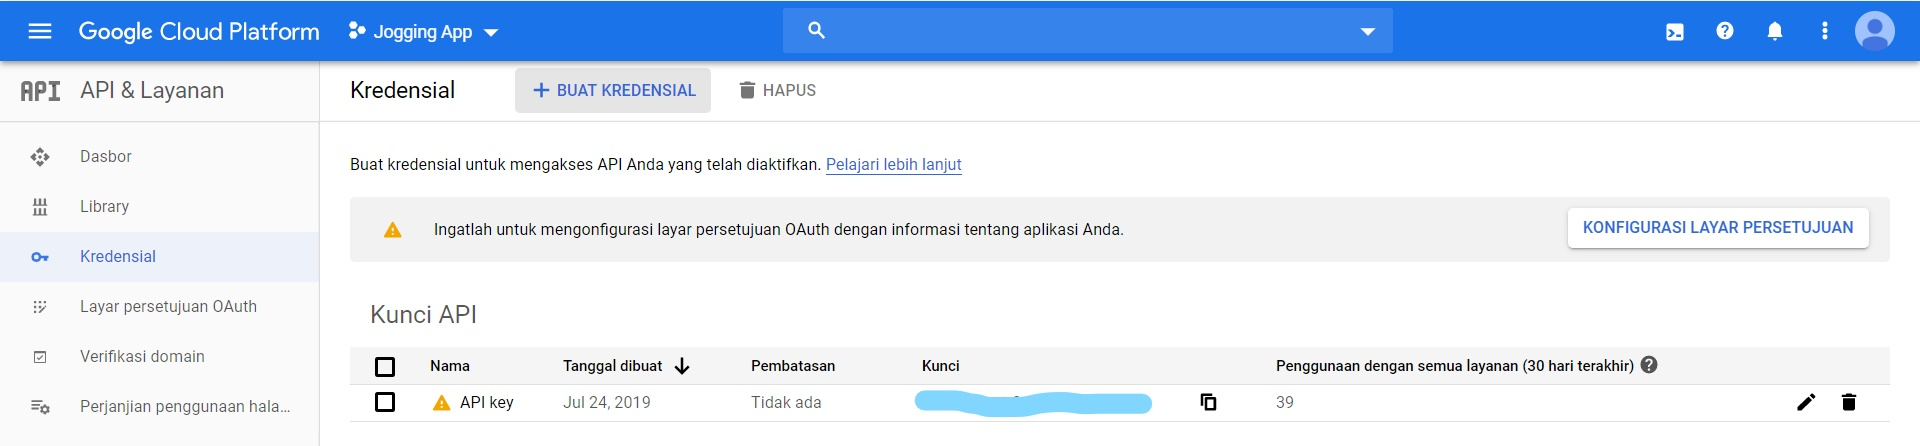
\includegraphics[width=6in]{Gambar/google_cloud.png}
	\caption{Tampilan \textit{UI Google Cloud} saat mengakses \textit{API Key} (\textit{API Key disamarkan})}
	\label{fig:googlecloud}
\end{figure}

\subsection{{\it API Key}}
\label{subs:api-key}
Agar dapat menggunakan {\it StreetView API} (dan \textit{Directions API} pada Subbab \ref{sec:directions}), ada {\it API key} yang harus diperoleh pada Google Cloud Platform Console dengan memasukkan nomor kartu kredit. Gambar \ref{fig:googlecloud} menunjukkan tampilan \textit{Google Cloud} setelah mendapatkan API key ~\cite{api-key}. API {\it key} yang diberikan terdiri atas dua puluh dan delapan belas karakter alfanumerik (bisa huruf kapital dan huruf kecil) yang dihubungkan dengan tanda "-". API {\it key} yang telah diperoleh akan digunakan sebagai salah satu parameter masukan agar Google API dapat diakses.

%\subsection{Atribut \textit{location}}
%\label{subs:location-attr}
%Salah satu Atribut yang sering digunakan untuk menggunakan \textit{StreetView API} (dan \texit{Directions API} pada Subbab \ref{sec:directions}) adalah \textit{location}. Ada beberapa jenis parameter yang diterima untuk atribut \textit{location}, di antaranya:
%\begin{itemize}
%	\item Garis lintang dan garis bujur (\textit{longitude} dan \textit{latitude}.
%	\item place
%\end{itemize} 

\subsection{Penggunaan {\it StreetView API}}
\label{subs:streetview-usage}
Secara umum, API diakses menggunakan URL Web sebagai berikut:
\begin{quote}
https://maps.googleapis.com/maps/api/streetview?parameters
\end{quote}
"Parameters" pada URL Web adalah atribut-atribut dengan parameter yang diterima StreetView. Sintaks parameter tersebut adalah: $$ X = Y $$
X adalah atribut dari StreetView, sedangkan Y adalah nilainya, dan nilai tersebut harus sesuai dengan tipe dan rentang nilai masing-masing atribut. Untuk atribut kedua dan seterusnya yang akan dimasukkan dalam parameter (jika ada), dapat diteruskan dengan tanda "\&", lalu diikuti dengan pola seperti rumus di atas. Saat mengakses {\it StreetView API}, ada dua kemungkinan hasil yang diperoleh, yaitu berhasil dan gagal. Pemanggilan \textit{API} yang berhasil akan menghasilkan gambar pemandangan dari lokasi sesuai masukan pengguna, sementara pemanggilan yang gagal menghasilkan sebuah gambar dengan penjelasan bahwa gambar tidak tersedia. 

%Gambar \ref{fig:success-streetview} memperlihatkan pemanggilan \textit{StreetView API} yang berhasil.

\subsection{Atribut Parameter {\it StreetView API}}
\label{subs:parameter}
Untuk menampilkan pemandangan yang sesuai keinginan pengguna, beberapa parameter masukan harus ditentukan. Ada dua jenis parameter masukan, di antaranya parameter wajib dan parameter opsional. Pengaksesan atau pemanggilan {\it StreetView API} yang berhasil akan mengembalikan sebuah gambar pemandangan dari lokasi sesuai parameter masukan. 

\subsubsection{Parameter Wajib}
Parameter wajib adalah parameter yang harus dimasukkan oleh pengguna dan jika tidak dimasukkan akan mengakibatkan pemanggilan yang gagal. 
Beberapa parameter wajib pada {\it StreetView API} adalah:
\begin{itemize}
	\item \textit{size}
		
	Ukuran dari gambar yang dihasilkan, dalam \textit{pixel}. Format parameter adalah:
	 banyak \textit{pixel} secara horisontal $\times$ banyak \textit{pixel} secara vertikal.
	\item \textit{key}
	
	\textit{API key} yang dijelaskan pada Subbab \ref{subs:api-key}.
	\item \textit{location} atau \textit{pano} (salah satu)
	 
	 Lokasi dari pemandangan yang ingin ditampilkan. \textit{locaction} menerima dua jenis parameter garis lintang dan garis bujur (\textit{longitude} dan \textit{latitude}) atau \textit{String} nama lokasi, sementara \textit{pano} menerima \textit{panorama id} dari lokasi atau panorama. 
	 
\end{itemize}   

\subsubsection{Parameter Opsional}
Selain parameter wajib, ada parameter opsional, yaitu parameter yang tidak perlu diisi agar pengaksesan {\it API} berhasil dan biasanya atribut parameter tersebut sudah memiliki nilai bawaan ({\it default}). Ada beberapa parameter opsional yang dapat digunakan sebagai parameter untuk mengubah pengaturan dari pemandangan yang diambil:
\begin{itemize}
	\item {\it signature}
	
	Atribut untuk memastikan bahwa \textit{request} dikirim dengan {\it API key} sesuai jenis \textit{signature} yang diatur pemilik {\it API key}. Nilai dari \textit{signature} bertipe alfabetik.
	\item {\it heading}
	
	Atribut yang menyatakan arah pandangan secara horisontal, nilai atribut menyatakan sudut yang dibentuk dari arah utara dengan arah pandang yang diinginkan (sudut yang dibentuk dari arah berlawanan jarum jam), dengan rentang bilangan bulat positif.
	\item {\it fov} ({\it field of view})
	
	Atribut yang menyatakan seberapa perbesaran pemandangan (nilai dalam satuan derajat dengan rentang nilai 10 sammpai 120).
	\item {\it pitch}
	
	Atribut yang menyatakan pandangan pengguna secara vertikal, satuan nilai dalam derajat, dengan rentang nilai bilangan bulat dari -90 sampai 90.
	\item {\it radius} 
	
	Atribut yang menyatakan jarak dalam meter, yang adalah titik pengambilan pemandangan, dengan rentang nilai bilangan bulat positif dan nol. 
	\item {\it source}
	
	Atribut yang menyatakan jenis pemandangan, \textit{default} atau \textit{outdoor} (bertipe data alfabetik).
\end{itemize}
    

\subsubsection{Hasil Pemanggilan \textit{StreetView API}}
Pemanggilan \textit{StreetView} yang berrhasil akan menghasilkan sebuah gambar dari pemandangan sesuai lokasi. Gambar \ref{fig:success-streetview} memperlihatkan pemanggilan \textit{StreetView API} yang berhasil dengan \textit{URL} \url{https://maps.googleapis.com/maps/api/streetview?size=600x300\&location=-6.8746537,107.6046282\&key=(disamarkan)}.
\begin{figure}[h]
		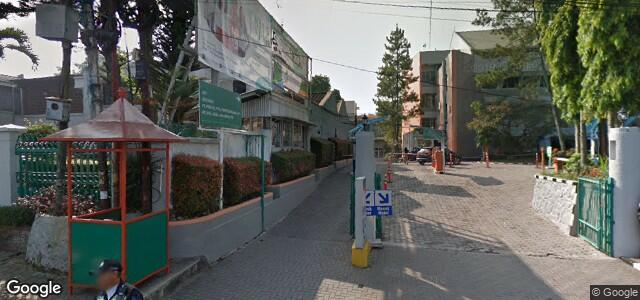
\includegraphics[scale=0.8]{Gambar/streetview90.png}
	\caption{Pemanggilan \textit{StreetView API} yang berhasil}
	\label{fig:success-streetview}
\end{figure}

%DIRECTIONS API
\section{Google {\it Directions API}}
\label{sec:directions}
Google {\it Directions API} adalah layanan berbasis \textit{HTTP}/\textit{HTTPS} dari Google yang membantu mencari dan menghitung arah dari satu tempat ke tempat yang lain ~\cite{directions-api}. Ada beberapa \textit{mode} dari arah yang dapat dicari seperti {\it driving}, {\it transit}, {\it walking}, dan {\it cycling}. Pengaksesan \textit{Directions API} sangat mirip dengan {\it StreetView API}, yaitu membutuhkan \textit{API Key}, seperti yang dijelaskan pada Subbab \ref{subs:api-key}, sebagai salah satu atribut wajib, juga memiliki atribut wajib dan opsional yang dapat diatur lewat parameter. 

\subsection{Penggunaan {\it Directions API}}
Sintaks untuk mengaksesnya pun mirip dengan \textit{StreetView API} dengan \textit{URL} sebagai berikut:
\begin{quote}
https://maps.googleapis.com/maps/api/directions/filetype?parameter
\end{quote}
Bagian "filetype" pada \textit{URL} diganti dengan tipe \textit{file} keluaran atau hasil (xml atau json). Bagian "parameter" diganti dengan parameter-parameter dari {\it Directions API}.  {\it Directions API} juga memiliki dua jenis parameter seperti {\it StreetView API}: wajib dan opsional. Parameter-parameter tersebut di antaranya:

\begin{itemize}
	\item \textit{origin}
	
	Parameter wajib bertipe alfabetik yang menyatakan lokasi asal yang dimasukkan pengguna. Parameter ini diisi \textit{string} lokasi yang \textit{sah}.
	\item \textit{destination}
	
	Parameter wajib bertipe string alfabetik yang menyatakan lokasi yang valid dari lokasi tujuan yang dimasukkan pengguna.
	\item \textit{key}
	
	Parameter wajib yang bertipe String yang menyatakan \textit{API key} milik pengguna (seperti pada Subbab \ref{subs:api-key}).
	\item \textit{mode}
	
	Parameter opsional yang bertipe String yang menyatakan \textit{mode} perjalanan yang akan ditempuh, seperti "\textit{driving}", "\textit{walking}", "\textit{bicycling}", atau "\textit{transit}"
	\item \textit{waypoints}
	
	Parameter opsional yang menyatakan lokasi yang ingin ditempuh dalam perjalanan. Parameter ini dapat diisi dengan beberapa jenis parameter yang menyatakan lokasi seperti garis lintang dan garis bujur dan \textit{string} alamat lokasi.
	\item \textit{alternatives}
	
	Parameter opsional \textit{bit} (\textit{boolean}) yang menyatakan apakah rute yang disediakan \textit{Directions API} menyediakan beberapa pilihan rute atau tidak. 
	\item \textit{avoid}
	
	Parameter opsional bertipe \textit{String} (alfabetik) yang menyatakan jenis-jenis jalan yang harus dihindari. Nilai-nilai yang sah untuk parameter ini adalah "\textit{tolls}", "\textit{highways}", "\textit{ferries}, dan/atau "\textit{indoor}" (nilai dipisahkan dengan "|" jika ada beberapa).
	\item \textit{language}
	
	Parameter opsional bertipe \textit{string} (alfabetik) yang menyatakan bahasa yang digunakan untuk menyajikan rute perjalanan sesuai bahasa yang disediakan Google. 
	\item \textit{units}
	
	Parameter opsional bertipe \textit{String} (alfabetik) yang menyatakan jenis satuan yang akan digunakan, seperti "\textit{metrics}" atau "\textit{imperial}".
	\item \textit{region}
	
	Parameter opsional terdiri dari dua karaketer yang menyatakan kode daerah.
	\item \textit{arrival\_time} 
	
	Parameter opsional bertipe bilangan bulat yang menandakan waktu yang diinginkan untuk sampai di tujuan.
	\item \textit{departure\_time} 
	
	Parameter opsional bertipe bilangan bulat yang menyatakan waktu keberangkatan yang diinginkan.
	\item \textit{traffic\_model}
	
	Parameter opsional \textit{string} (alfabetik) yang menyatakan jenis perjalanan yang disajikan sesuai waktu tempuh, seperti perjalanan dengan waktu paling tepat ("\textit{best\_guess}"), yang paling optimis ("\textit{optimistic}"), dan yang paling pesimis ("\textit{pessimistic}").
	
\end{itemize}


\subsection{Hasil Pemanggilan \textit{Directions API}}
Hal yang dihasilkan oleh pemanggilan \textit{Directions API} adalah \textit{script} Javascript Notation Object (JSON) yang menyatakan arah sesuai lokasi asal dan tujuan, serta mode perjalanan yang adalah masukan pengguna ~\cite{directions-api}. Selain arah, \textit{script} JSON yang dikembalikan juga mengandung informasi mengenai jarak jalan yang ditempuh serta waktu tempuh perjalanan. Listing \ref{list:success_directions} menunjukkan contoh \textit{script} JSON dengan \textit{URL} \url{https://maps.googleapis.com/maps/api/directions/json?origin=unpar&destination=Rumah+Sakit+Santo+Borromeus&mode=walking&key=...} (parameter \textit{key} tidak dicantumkan). Pemanggilan yang gagal akan mengembalikan \textit{script} JSON yang menyatakan jalan di antara dua lokasi masukan tidak dapat ditemukan.


\begin{lstlisting}[caption={Hasil Pemanggilan \textit{Directions API} yang Berhasil},label={list:success_directions},language=java]
{
   "geocoded_waypoints" : [
      {
         "geocoder_status" : "OK",
         "place_id" : "ChIJbYmcEu7maC4RRijB2oKhHLA",
         "types" : [ "establishment", "point_of_interest", "university" ]
      },
      {
         "geocoder_status" : "OK",
         "place_id" : "ChIJU8k7DlHmaC4RQ2mUo1ERm1k",
         "types" : [ "establishment", "health", "hospital", "point_of_interest" ]
      }
   ],
   "routes" : [
      {
         "bounds" : {
            "northeast" : {
               "lat" : -6.8746719,
               "lng" : 107.6137497
            },
            "southwest" : {
               "lat" : -6.893148,
               "lng" : 107.6034915
            }
         },
         "copyrights" : "Map data c2020",
         "legs" : [
            {
               "distance" : {
                  "text" : "3.0 km",
                  "value" : 2980
               },
               "duration" : {
                  "text" : "35 mins",
                  "value" : 2116
               },
               "end_address" : "Jl. Ir. H. Juanda No.100, Lebakgede...",
               "end_location" : {
                  "lat" : -6.893148,
                  "lng" : 107.6131791
               },
               "start_address" : "Jl. Ciumbuleuit No.94, Hegarmanah...",
               "start_location" : {
                  "lat" : -6.8746719,
                  "lng" : 107.6046127
               },
               "steps" : [
                  {
                     "distance" : {
                        "text" : "1.0 km",
                        "value" : 1008
                     },
                     "duration" : {
                        "text" : "11 mins",
                        "value" : 667
                     },
                     "end_location" : {
                        "lat" : -6.8833328,
                        "lng" : 107.6049108
                     },
                     "html_instructions" : "Head \u003cb\u003esouth...",
                     "polyline" : {
                        "points" : "tu}h@yowoSdAP|AL`Cb@dAHHBvC..."
                     },
                     "start_location" : {
                        "lat" : -6.8746719,
                        "lng" : 107.6046127
                     },
                     "travel_mode" : "WALKING"
                  },
                  {
                     "distance" : {
                        "text" : "1.1 km",
                        "value" : 1078
                     },
                     "duration" : {
                        "text" : "14 mins",
                        "value" : 834
                     },
                     "end_location" : {
                        "lat" : -6.885218399999999,
                        "lng" : 107.6137497
                     },
                     "html_instructions" : "Turn \u003cb\u003eleft\u003c/b...",
                     "maneuver" : "turn-left",
                     "polyline" : {
                        "points" : "xk_i@uqwoSCEAECKAM?K?E?..."
                     },
                     "start_location" : {
                        "lat" : -6.8833328,
                        "lng" : 107.6049108
                     },
                     "travel_mode" : "WALKING"
                  },
                  {
                     "distance" : {
                        "text" : "0.9 km",
                        "value" : 884
                     },
                     "duration" : {
                        "text" : "10 mins",
                        "value" : 603
                     },
                     "end_location" : {
                        "lat" : -6.893140799999999,
                        "lng" : 107.6130843
                     },
                     "html_instructions" : "Turn \u003cb\u003eright...",
                     "maneuver" : "turn-right",
                     "polyline" : {
                        "points" : "rw_i@}hyoSzCLlAHz@Bd@@fB@tBDfABR@L..."
                     },
                     "start_location" : {
                        "lat" : -6.885218399999999,
                        "lng" : 107.6137497
                     },
                     "travel_mode" : "WALKING"
                  },
                  {
                     "distance" : {
                        "text" : "10 m",
                        "value" : 10
                     },
                     "duration" : {
                        "text" : "1 min",
                        "value" : 12
                     },
                     "end_location" : {
                        "lat" : -6.893148,
                        "lng" : 107.6131791
                     },
                     "html_instructions" : "Turn \u003cb\u003eleft\u003c...",
                     "maneuver" : "turn-left",
                     "polyline" : {
                        "points" : "biai@wdyoS@S"
                     },
                     "start_location" : {
                        "lat" : -6.893140799999999,
                        "lng" : 107.6130843
                     },
                     "travel_mode" : "WALKING"
                  }
               ],
               "traffic_speed_entry" : [],
               "via_waypoint" : []
            }
         ],
         "overview_polyline" : {
            "points" : "tu}h@yowoSdAP|AL`Cb@dAH`Dd@~Bd@hG..."
         },
         "summary" : "Jl. Ciumbuleuit, Jl. Siliwangi...",
         "warnings" : [
            "Walking directions are in beta. Use caution..."
         ],
         "waypoint_order" : []
      }
   ],
   "status" : "OK"
}
\end{lstlisting}

Penjelasan mengenai atribut-atribut hasil keluaran \textit{Directions API} adalah sebagai berikut:

\begin{itemize}
	\item \textit{geocoded\_waypoints}
	
	Berisi kumpulan rincian lokasi asal, tujuan, dan \textit{waypoint}-\textit{waypoint} yang ditentukan pengguna (rincian termasuk \textit{id} dan jenis tempat). Masing-masing objek dalam atribut ini memiliki atribut-atribut:
	
	\begin{itemize}
		\item \textit{geocoder\_status}
		
		Status keabsahan tempat. 
		\item \textit{place\_id}
		
		\textit{String} alfanumerik dari \textit{id} tempat.
		\item \textit{types}
		
		\textit{Array} dari deskripsi tempat, seperti kantor, pusat kesehatan, bangunan, dan sebagainya. 
	\end{itemize}
	\item \textit{routes}
	
	\textit{Array} dari jalan-jalan yang merupakan rute yang ditempuh dari lokasi asal ke lokasi tujuan. Setiap objek dari atribut ini memiliki atribut-atribut:
	
	\begin{itemize}
		
		\item \textit{copyrights}
		
		\textit{Copyright text} yang ditunjukkan untuk suatu jalan.
		\item \textit{legs}[]
		
		\textit{Array} dari satu \textit{leg}, yang adalah objek yang mengandung informasi mengenai jalan yang ditempuh. Setiap objek \textit{leg} memiliki atribut-atribut:
		
		\begin{itemize}
			\item \textit{distance}
			
			Panjang dari jalan yang dilewati.
			\item \textit{duration}
			
			Lama waktu yang dibutuhkan untuk menempuh jalan sesuai \textit{mode}.
			\item \textit{start\_address}
			
			Alamat dari satu titik ujung dari jalan yang ditempuh terlebih dahulu pada perjalanan.
			\item \textit{start\_location}			
			
			Koordinat garis lintang dan garis bujur dari \textit{start\_address}.
			\item \textit{end\_address}
			
			Alamat dari satu titik ujung dari jalan yang ditempuh kemudian atau terakhir pada perjalanan.
			\item \textit{end\_location}
			
			Koordinat garis lintang dan garis bujur dari \textit{end\_address}.
			
		\end{itemize}				
		
		\item \textit{overview\_polyline}
		
		Satu objek \textit{point} yang merupakan representasi rute. 
		\item \textit{bounds}
		
		\textit{Viewport} pembatas dari lokasi.
		\item \textit{summary}
		
		Deskripsi dari jalur seperti arah yang diambil. 
		\item \textit{warnings}[]
		
		\textit{Array} yang berisi peringatan saat rute perjalanan ditampilkan. 
		\item \textit{waypoint\_order}
		
		\textit{Array} dari urutan \textit{waypoint} yang dilewati.
	\end{itemize}
	\item \textit{status}
	
	Berisi status dari \textit{request} pengaksesan \textit{Directions API}.
\end{itemize}

%SENSOR
\section{\textit{Motion Sensor}}
\label{subs:motion-sensor}

\subsection{Deskripsi \textit{Motion Sensor}}
\textit{Motion sensor} adalah sensor pada \textit{smartphone} yang mendeteksi pergerakan gawai \textit{smartphone} ~\cite{motion-sensor}. Pergerakan yang dapat dideteksi termasuk saat gawai dimiringkan, digoyangkan, diayunkan, atau diputar (sumber). Beberapa contoh \textit{motion sensor} pada \textit{smartphone} adalah:
\begin{itemize}
	\item \textit{accelerometer}
	
	Sensor yang mendeteksi gerakan \textit{smartphone} terhadap sumbu $x, y,$ dan $z$, termasuk gaya gravitasi terhadap masing-masing sumbu.
	\item \textit{gravity sensor}
	
	Sensor yang mendeteksi gaya gravitasi terhadap sumbu $x, y,$ dan $z$.
	\item \textit{gyroscope}
	
	Sensor yang mendeteksi putaran gawai terhadap sumbu $x, y,$ dan $z$.
	\item \textit{linear acceleration sensor}
	
	Sensor yang mendeteksi pergerakan linier, terhadap sumbu $x, y,$ dan $z$ tanpa gaya gravitasi pada masing-masing sumbu.
	\item \textit{rotation vector sensor}
	
	Sensor yang mendeteksi vektor putaran pada gawai terhadap sumbu $x, y,$ dan $z$.
	
	\item \textit{step counter}
	
	Sensor yang menghitung jumlah langkah saat berjalan yang pengguna gawai ambil.
	\item \textit{step detector}
	
	Sensor yang men-\textit{trigger} sebuah \textit{event} saat pengguna mengambil langkah saat berjalan.
\end{itemize}

Sintaks untuk menggunakan sensor ini tertera pada Listing \ref{list:step_detector_syntax}.

\begin{lstlisting}[caption={Sintaks menggunakan sensor \textit{step detector}},label={list:step_detector_syntax},language=java]
private SensorManager sensorManager;
private Sensor sensor;
...
sensorManager = (SensorManager) getSystemService(Context.SENSOR_SERVICE);
sensor = sensorManager.getDefaultSensor(Sensor.TYPE_STEP_DETECTOR);
\end{lstlisting} 

\subsection{Deskripsi \textit{Step Detector}}
\textit{Step detector} adalah sensor yang digunakan untuk mendeteksi langkah kaki pengguna. Sensor ini dapat memicu suatu \textit{event} setiap kali langkah kaki pengguna diambil. Nilai yang dikembalikan adalah 1.0 dan \textit{timestamp} dari saat langkah kaki diambil pengguna (nilai 1.0 menunjukkan bahwa ada langkah yang telah diambil). \textit{Permission} yang dibutuhkan untuk mengaktifkan sensor ini adalah \texttt{android.permission.ACTIVITY\_RECOGNITION}. Latensi dari sensor ini sekitar kurang dari dua detik. 
